
% Aqui escribiré la introducción del tfg


\chapter*{Introducción}
\addcontentsline{toc}{chapter}{Introducción}


\spacedlowsmallcaps{Contexto}

Cuando en $1948$ Claude Shannon publicó ``Una teoría matemática sobre la comunicación"\ \cite{Shannon} empezó a surgir la teoría de la información. En dicha publicación, Shannon explica que en un sistema de comunicación es posible realizar una comunicación fiable si no sobrepasamos la capacidad del canal. Además, en el artículo se expone como ejemplo la corrección de un código de Hamming. Un par de años más tarde, en $1950$ Richard Hamming publicó ``Error detecting and error correcting codes"\ \cite{Hamming} y empezó a surgir la teoría de códigos. La motivación de esta publicación se debe a que en los ordenadores, un simple error supone un fallo completo en la tarea realizada, en el sentido de que si se detecta, no se puede seguir calculando hasta que se localice y corrija el fallo, mientras que si no se detecta, invalida todas las operaciones posteriores realizadas. Por ello, Hamming expone la importancia de detectar y corregir errores que se pueden producir al trabajar con grandes números y problemas complejos así como una construcción de códigos que resuelvan este problema.


Con la teoría de códigos queremos conseguir el envío seguro de mensajes, pudiendo codificarlos antes de enviarlos y decodificarlos al recibirlos, así el problema se encuentra en asegurarse que el mensaje recibido es el mismo que el enviado. Por ejemplo, no es práctico transmitir imágenes de planetas desde el espacio, ya que si alguna parte de los datos se ha modificado debido al ruido que haya en la transmisión, esos datos ya no nos servirían. El Teorema de Shannon nos garantiza que un cierto porcentaje de veces esto será cierto. Con un correcto decodificador este porcentaje se puede aumentar tanto como queramos aunque nunca llegará al $100$\%. La prueba del teorema es probabilística y no constructiva, es decir, que no produce ningún tipo específico de códigos, solo su existencia, por ello, el objetivo es encontrar códigos que cumplan las condiciones de este teorema.

En la figura \ref{fig:uno} podemos observar un canal de comunicación, en donde las flechas indican que la comunicación se produce en un único sentido. Supongamos ahora que un emisor le quiere enviar un mensaje $x = x_1 \cdots x_k$ compuesto por una secuencia finita de elementos de un alfabeto a un receptor, a través de un canal. Si no hiciésemos ninguna modificación al mensaje original, cualquier interferencia podría alterarlo de forma que no podríamos recuperarlo. La idea básica es añadir redundancia al mensaje durante la codificación para obtener una palabra código $c = c_1\cdots c_n$ que es la que se envía por el canal donde el ruido en forma de error $e=e_1 \cdots e_n$ la perturba y obtenemos $c' = c + e$. Esto es lo que enviamos al decodificador donde corregimos los errores,eliminamos la redundancia y obtenemos $x'$ que es el mensaje decodificado. Lo ideal es que $x' = x$. \cite{Huffman_Pless_2010}



\begin{figure}[H]

	\center
	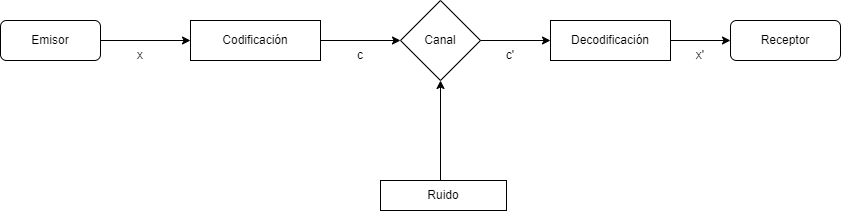
\includegraphics[scale=0.5]{img/canal_comunicacion.png}
	\caption{Canal de Comunicación, \cite{Podesta_2006}.}
     \label{fig:uno}
\end{figure}


La Teoría de Códigos Autocorrectores se ocupa del segundo y cuarto pasos del esquema anterior, es decir, de la codificación y decodificación de mensajes, junto con el problema de
detectar y corregir errores. A veces no es posible pedir retransmisión de mensajes y es por eso que los códigos autocorrectores son tan útiles y necesarios. \cite{Podesta_2006}


%\spacedlowsmallcaps{Estado del arte}



\spacedlowsmallcaps{Descripción y Estructura del proyecto}

Realizaremos una descripción del proyecto realizado a través de las diferentes partes que podemos distinguir en esta memoria:

El primer capítulo sirve como introducción a las herramientas y conceptos que van a ser utilizados frecuentemente a lo largo del resto de capítulos. Se recoge la teoría que será necesaria para el desarrollo del proyecto.

A continuación se presentan y explican los códigos lineales y cíclicos junto a sus propiedades. Analizamos las características necesarias y más relevantes para realizar una buena detección y correción de errores como es encontrar una cota para la distancia mínima de un código. Así, describiremos una familia de códigos cíclicos que tienen una cota muy conocida que es la cota BCH. Además, se realiza la decodificación de este tipo de códigos.

En el tercer capítulo se presenta el anillo de los polinomios torcidos con coeficientes en un cuerpo, cuya diferencia con el anillo de los polinomios usuales radica en el uso de un automorfismo del cuerpo que transforma la multiplicación y ya no es conmutativa. Por tanto, se observan diferencias tanto en la factorización de polinomios como en la evaluación de éstos. Se realiza un estudio de todas estas propiedades.

Durante el cuarto capítulo, utilizaremos la teoría vista en las anteriores secciones y la aplicaremos para conseguir un nuevo tipo de códigos que son los códigos torcidos. Se verá paso a paso la construcción de estos con ejemplos representativos. Además también definiremos la familia de los códigos Reed-Solomon torcidos y su ligera diferencia en construcción con los demás códigos torcidos. Finalmente, se estudia un algoritmo de decodificación para estos códigos y como se pueden corregir errores cometidos en el envío de mensajes.

Para terminar, en el último capítulo, se discutirán aspectos del trabajo, así como los objetivos alcanzados y mejoras a la memoria con el fin de seguir investigando en este campo. 




\spacedlowsmallcaps{Objetivos del trabajo}

En esta sección, se recogen los objetivos que se pretenden realizar en este trabajo.

\begin{itemize}
    \item Estudiar la teoría básica de códigos lineales y cíclicos.
    \item Estudiar el anillo de los polinomios torcidos.
    \item Estudiar los códigos Reed-Solomon torcidos.
    \item Estudiar el Algoritmo de Sugiyama y su implementación para códigos Reed-Solomon torcidos.    
\end{itemize}

